
% Default to the notebook output style

    


% Inherit from the specified cell style.




    
\documentclass[11pt]{article}

    
    
    \usepackage[T1]{fontenc}
    % Nicer default font (+ math font) than Computer Modern for most use cases
    \usepackage{mathpazo}

    % Basic figure setup, for now with no caption control since it's done
    % automatically by Pandoc (which extracts ![](path) syntax from Markdown).
    \usepackage{graphicx}
    % We will generate all images so they have a width \maxwidth. This means
    % that they will get their normal width if they fit onto the page, but
    % are scaled down if they would overflow the margins.
    \makeatletter
    \def\maxwidth{\ifdim\Gin@nat@width>\linewidth\linewidth
    \else\Gin@nat@width\fi}
    \makeatother
    \let\Oldincludegraphics\includegraphics
    % Set max figure width to be 80% of text width, for now hardcoded.
    \renewcommand{\includegraphics}[1]{\Oldincludegraphics[width=.8\maxwidth]{#1}}
    % Ensure that by default, figures have no caption (until we provide a
    % proper Figure object with a Caption API and a way to capture that
    % in the conversion process - todo).
    \usepackage{caption}
    \DeclareCaptionLabelFormat{nolabel}{}
    \captionsetup{labelformat=nolabel}

    \usepackage{adjustbox} % Used to constrain images to a maximum size 
    \usepackage{xcolor} % Allow colors to be defined
    \usepackage{enumerate} % Needed for markdown enumerations to work
    \usepackage{geometry} % Used to adjust the document margins
    \usepackage{amsmath} % Equations
    \usepackage{amssymb} % Equations
    \usepackage{textcomp} % defines textquotesingle
    % Hack from http://tex.stackexchange.com/a/47451/13684:
    \AtBeginDocument{%
        \def\PYZsq{\textquotesingle}% Upright quotes in Pygmentized code
    }
    \usepackage{upquote} % Upright quotes for verbatim code
    \usepackage{eurosym} % defines \euro
    \usepackage[mathletters]{ucs} % Extended unicode (utf-8) support
    \usepackage[utf8x]{inputenc} % Allow utf-8 characters in the tex document
    \usepackage{fancyvrb} % verbatim replacement that allows latex
    \usepackage{grffile} % extends the file name processing of package graphics 
                         % to support a larger range 
    % The hyperref package gives us a pdf with properly built
    % internal navigation ('pdf bookmarks' for the table of contents,
    % internal cross-reference links, web links for URLs, etc.)
    \usepackage{hyperref}
    \usepackage{longtable} % longtable support required by pandoc >1.10
    \usepackage{booktabs}  % table support for pandoc > 1.12.2
    \usepackage[inline]{enumitem} % IRkernel/repr support (it uses the enumerate* environment)
    \usepackage[normalem]{ulem} % ulem is needed to support strikethroughs (\sout)
                                % normalem makes italics be italics, not underlines
    

    
    
    % Colors for the hyperref package
    \definecolor{urlcolor}{rgb}{0,.145,.698}
    \definecolor{linkcolor}{rgb}{.71,0.21,0.01}
    \definecolor{citecolor}{rgb}{.12,.54,.11}

    % ANSI colors
    \definecolor{ansi-black}{HTML}{3E424D}
    \definecolor{ansi-black-intense}{HTML}{282C36}
    \definecolor{ansi-red}{HTML}{E75C58}
    \definecolor{ansi-red-intense}{HTML}{B22B31}
    \definecolor{ansi-green}{HTML}{00A250}
    \definecolor{ansi-green-intense}{HTML}{007427}
    \definecolor{ansi-yellow}{HTML}{DDB62B}
    \definecolor{ansi-yellow-intense}{HTML}{B27D12}
    \definecolor{ansi-blue}{HTML}{208FFB}
    \definecolor{ansi-blue-intense}{HTML}{0065CA}
    \definecolor{ansi-magenta}{HTML}{D160C4}
    \definecolor{ansi-magenta-intense}{HTML}{A03196}
    \definecolor{ansi-cyan}{HTML}{60C6C8}
    \definecolor{ansi-cyan-intense}{HTML}{258F8F}
    \definecolor{ansi-white}{HTML}{C5C1B4}
    \definecolor{ansi-white-intense}{HTML}{A1A6B2}

    % commands and environments needed by pandoc snippets
    % extracted from the output of `pandoc -s`
    \providecommand{\tightlist}{%
      \setlength{\itemsep}{0pt}\setlength{\parskip}{0pt}}
    \DefineVerbatimEnvironment{Highlighting}{Verbatim}{commandchars=\\\{\}}
    % Add ',fontsize=\small' for more characters per line
    \newenvironment{Shaded}{}{}
    \newcommand{\KeywordTok}[1]{\textcolor[rgb]{0.00,0.44,0.13}{\textbf{{#1}}}}
    \newcommand{\DataTypeTok}[1]{\textcolor[rgb]{0.56,0.13,0.00}{{#1}}}
    \newcommand{\DecValTok}[1]{\textcolor[rgb]{0.25,0.63,0.44}{{#1}}}
    \newcommand{\BaseNTok}[1]{\textcolor[rgb]{0.25,0.63,0.44}{{#1}}}
    \newcommand{\FloatTok}[1]{\textcolor[rgb]{0.25,0.63,0.44}{{#1}}}
    \newcommand{\CharTok}[1]{\textcolor[rgb]{0.25,0.44,0.63}{{#1}}}
    \newcommand{\StringTok}[1]{\textcolor[rgb]{0.25,0.44,0.63}{{#1}}}
    \newcommand{\CommentTok}[1]{\textcolor[rgb]{0.38,0.63,0.69}{\textit{{#1}}}}
    \newcommand{\OtherTok}[1]{\textcolor[rgb]{0.00,0.44,0.13}{{#1}}}
    \newcommand{\AlertTok}[1]{\textcolor[rgb]{1.00,0.00,0.00}{\textbf{{#1}}}}
    \newcommand{\FunctionTok}[1]{\textcolor[rgb]{0.02,0.16,0.49}{{#1}}}
    \newcommand{\RegionMarkerTok}[1]{{#1}}
    \newcommand{\ErrorTok}[1]{\textcolor[rgb]{1.00,0.00,0.00}{\textbf{{#1}}}}
    \newcommand{\NormalTok}[1]{{#1}}
    
    % Additional commands for more recent versions of Pandoc
    \newcommand{\ConstantTok}[1]{\textcolor[rgb]{0.53,0.00,0.00}{{#1}}}
    \newcommand{\SpecialCharTok}[1]{\textcolor[rgb]{0.25,0.44,0.63}{{#1}}}
    \newcommand{\VerbatimStringTok}[1]{\textcolor[rgb]{0.25,0.44,0.63}{{#1}}}
    \newcommand{\SpecialStringTok}[1]{\textcolor[rgb]{0.73,0.40,0.53}{{#1}}}
    \newcommand{\ImportTok}[1]{{#1}}
    \newcommand{\DocumentationTok}[1]{\textcolor[rgb]{0.73,0.13,0.13}{\textit{{#1}}}}
    \newcommand{\AnnotationTok}[1]{\textcolor[rgb]{0.38,0.63,0.69}{\textbf{\textit{{#1}}}}}
    \newcommand{\CommentVarTok}[1]{\textcolor[rgb]{0.38,0.63,0.69}{\textbf{\textit{{#1}}}}}
    \newcommand{\VariableTok}[1]{\textcolor[rgb]{0.10,0.09,0.49}{{#1}}}
    \newcommand{\ControlFlowTok}[1]{\textcolor[rgb]{0.00,0.44,0.13}{\textbf{{#1}}}}
    \newcommand{\OperatorTok}[1]{\textcolor[rgb]{0.40,0.40,0.40}{{#1}}}
    \newcommand{\BuiltInTok}[1]{{#1}}
    \newcommand{\ExtensionTok}[1]{{#1}}
    \newcommand{\PreprocessorTok}[1]{\textcolor[rgb]{0.74,0.48,0.00}{{#1}}}
    \newcommand{\AttributeTok}[1]{\textcolor[rgb]{0.49,0.56,0.16}{{#1}}}
    \newcommand{\InformationTok}[1]{\textcolor[rgb]{0.38,0.63,0.69}{\textbf{\textit{{#1}}}}}
    \newcommand{\WarningTok}[1]{\textcolor[rgb]{0.38,0.63,0.69}{\textbf{\textit{{#1}}}}}
    
    
    % Define a nice break command that doesn't care if a line doesn't already
    % exist.
    \def\br{\hspace*{\fill} \\* }
    % Math Jax compatability definitions
    \def\gt{>}
    \def\lt{<}
    % Document parameters
    \title{week1}
    
    
    

    % Pygments definitions
    
\makeatletter
\def\PY@reset{\let\PY@it=\relax \let\PY@bf=\relax%
    \let\PY@ul=\relax \let\PY@tc=\relax%
    \let\PY@bc=\relax \let\PY@ff=\relax}
\def\PY@tok#1{\csname PY@tok@#1\endcsname}
\def\PY@toks#1+{\ifx\relax#1\empty\else%
    \PY@tok{#1}\expandafter\PY@toks\fi}
\def\PY@do#1{\PY@bc{\PY@tc{\PY@ul{%
    \PY@it{\PY@bf{\PY@ff{#1}}}}}}}
\def\PY#1#2{\PY@reset\PY@toks#1+\relax+\PY@do{#2}}

\expandafter\def\csname PY@tok@w\endcsname{\def\PY@tc##1{\textcolor[rgb]{0.73,0.73,0.73}{##1}}}
\expandafter\def\csname PY@tok@c\endcsname{\let\PY@it=\textit\def\PY@tc##1{\textcolor[rgb]{0.25,0.50,0.50}{##1}}}
\expandafter\def\csname PY@tok@cp\endcsname{\def\PY@tc##1{\textcolor[rgb]{0.74,0.48,0.00}{##1}}}
\expandafter\def\csname PY@tok@k\endcsname{\let\PY@bf=\textbf\def\PY@tc##1{\textcolor[rgb]{0.00,0.50,0.00}{##1}}}
\expandafter\def\csname PY@tok@kp\endcsname{\def\PY@tc##1{\textcolor[rgb]{0.00,0.50,0.00}{##1}}}
\expandafter\def\csname PY@tok@kt\endcsname{\def\PY@tc##1{\textcolor[rgb]{0.69,0.00,0.25}{##1}}}
\expandafter\def\csname PY@tok@o\endcsname{\def\PY@tc##1{\textcolor[rgb]{0.40,0.40,0.40}{##1}}}
\expandafter\def\csname PY@tok@ow\endcsname{\let\PY@bf=\textbf\def\PY@tc##1{\textcolor[rgb]{0.67,0.13,1.00}{##1}}}
\expandafter\def\csname PY@tok@nb\endcsname{\def\PY@tc##1{\textcolor[rgb]{0.00,0.50,0.00}{##1}}}
\expandafter\def\csname PY@tok@nf\endcsname{\def\PY@tc##1{\textcolor[rgb]{0.00,0.00,1.00}{##1}}}
\expandafter\def\csname PY@tok@nc\endcsname{\let\PY@bf=\textbf\def\PY@tc##1{\textcolor[rgb]{0.00,0.00,1.00}{##1}}}
\expandafter\def\csname PY@tok@nn\endcsname{\let\PY@bf=\textbf\def\PY@tc##1{\textcolor[rgb]{0.00,0.00,1.00}{##1}}}
\expandafter\def\csname PY@tok@ne\endcsname{\let\PY@bf=\textbf\def\PY@tc##1{\textcolor[rgb]{0.82,0.25,0.23}{##1}}}
\expandafter\def\csname PY@tok@nv\endcsname{\def\PY@tc##1{\textcolor[rgb]{0.10,0.09,0.49}{##1}}}
\expandafter\def\csname PY@tok@no\endcsname{\def\PY@tc##1{\textcolor[rgb]{0.53,0.00,0.00}{##1}}}
\expandafter\def\csname PY@tok@nl\endcsname{\def\PY@tc##1{\textcolor[rgb]{0.63,0.63,0.00}{##1}}}
\expandafter\def\csname PY@tok@ni\endcsname{\let\PY@bf=\textbf\def\PY@tc##1{\textcolor[rgb]{0.60,0.60,0.60}{##1}}}
\expandafter\def\csname PY@tok@na\endcsname{\def\PY@tc##1{\textcolor[rgb]{0.49,0.56,0.16}{##1}}}
\expandafter\def\csname PY@tok@nt\endcsname{\let\PY@bf=\textbf\def\PY@tc##1{\textcolor[rgb]{0.00,0.50,0.00}{##1}}}
\expandafter\def\csname PY@tok@nd\endcsname{\def\PY@tc##1{\textcolor[rgb]{0.67,0.13,1.00}{##1}}}
\expandafter\def\csname PY@tok@s\endcsname{\def\PY@tc##1{\textcolor[rgb]{0.73,0.13,0.13}{##1}}}
\expandafter\def\csname PY@tok@sd\endcsname{\let\PY@it=\textit\def\PY@tc##1{\textcolor[rgb]{0.73,0.13,0.13}{##1}}}
\expandafter\def\csname PY@tok@si\endcsname{\let\PY@bf=\textbf\def\PY@tc##1{\textcolor[rgb]{0.73,0.40,0.53}{##1}}}
\expandafter\def\csname PY@tok@se\endcsname{\let\PY@bf=\textbf\def\PY@tc##1{\textcolor[rgb]{0.73,0.40,0.13}{##1}}}
\expandafter\def\csname PY@tok@sr\endcsname{\def\PY@tc##1{\textcolor[rgb]{0.73,0.40,0.53}{##1}}}
\expandafter\def\csname PY@tok@ss\endcsname{\def\PY@tc##1{\textcolor[rgb]{0.10,0.09,0.49}{##1}}}
\expandafter\def\csname PY@tok@sx\endcsname{\def\PY@tc##1{\textcolor[rgb]{0.00,0.50,0.00}{##1}}}
\expandafter\def\csname PY@tok@m\endcsname{\def\PY@tc##1{\textcolor[rgb]{0.40,0.40,0.40}{##1}}}
\expandafter\def\csname PY@tok@gh\endcsname{\let\PY@bf=\textbf\def\PY@tc##1{\textcolor[rgb]{0.00,0.00,0.50}{##1}}}
\expandafter\def\csname PY@tok@gu\endcsname{\let\PY@bf=\textbf\def\PY@tc##1{\textcolor[rgb]{0.50,0.00,0.50}{##1}}}
\expandafter\def\csname PY@tok@gd\endcsname{\def\PY@tc##1{\textcolor[rgb]{0.63,0.00,0.00}{##1}}}
\expandafter\def\csname PY@tok@gi\endcsname{\def\PY@tc##1{\textcolor[rgb]{0.00,0.63,0.00}{##1}}}
\expandafter\def\csname PY@tok@gr\endcsname{\def\PY@tc##1{\textcolor[rgb]{1.00,0.00,0.00}{##1}}}
\expandafter\def\csname PY@tok@ge\endcsname{\let\PY@it=\textit}
\expandafter\def\csname PY@tok@gs\endcsname{\let\PY@bf=\textbf}
\expandafter\def\csname PY@tok@gp\endcsname{\let\PY@bf=\textbf\def\PY@tc##1{\textcolor[rgb]{0.00,0.00,0.50}{##1}}}
\expandafter\def\csname PY@tok@go\endcsname{\def\PY@tc##1{\textcolor[rgb]{0.53,0.53,0.53}{##1}}}
\expandafter\def\csname PY@tok@gt\endcsname{\def\PY@tc##1{\textcolor[rgb]{0.00,0.27,0.87}{##1}}}
\expandafter\def\csname PY@tok@err\endcsname{\def\PY@bc##1{\setlength{\fboxsep}{0pt}\fcolorbox[rgb]{1.00,0.00,0.00}{1,1,1}{\strut ##1}}}
\expandafter\def\csname PY@tok@kc\endcsname{\let\PY@bf=\textbf\def\PY@tc##1{\textcolor[rgb]{0.00,0.50,0.00}{##1}}}
\expandafter\def\csname PY@tok@kd\endcsname{\let\PY@bf=\textbf\def\PY@tc##1{\textcolor[rgb]{0.00,0.50,0.00}{##1}}}
\expandafter\def\csname PY@tok@kn\endcsname{\let\PY@bf=\textbf\def\PY@tc##1{\textcolor[rgb]{0.00,0.50,0.00}{##1}}}
\expandafter\def\csname PY@tok@kr\endcsname{\let\PY@bf=\textbf\def\PY@tc##1{\textcolor[rgb]{0.00,0.50,0.00}{##1}}}
\expandafter\def\csname PY@tok@bp\endcsname{\def\PY@tc##1{\textcolor[rgb]{0.00,0.50,0.00}{##1}}}
\expandafter\def\csname PY@tok@fm\endcsname{\def\PY@tc##1{\textcolor[rgb]{0.00,0.00,1.00}{##1}}}
\expandafter\def\csname PY@tok@vc\endcsname{\def\PY@tc##1{\textcolor[rgb]{0.10,0.09,0.49}{##1}}}
\expandafter\def\csname PY@tok@vg\endcsname{\def\PY@tc##1{\textcolor[rgb]{0.10,0.09,0.49}{##1}}}
\expandafter\def\csname PY@tok@vi\endcsname{\def\PY@tc##1{\textcolor[rgb]{0.10,0.09,0.49}{##1}}}
\expandafter\def\csname PY@tok@vm\endcsname{\def\PY@tc##1{\textcolor[rgb]{0.10,0.09,0.49}{##1}}}
\expandafter\def\csname PY@tok@sa\endcsname{\def\PY@tc##1{\textcolor[rgb]{0.73,0.13,0.13}{##1}}}
\expandafter\def\csname PY@tok@sb\endcsname{\def\PY@tc##1{\textcolor[rgb]{0.73,0.13,0.13}{##1}}}
\expandafter\def\csname PY@tok@sc\endcsname{\def\PY@tc##1{\textcolor[rgb]{0.73,0.13,0.13}{##1}}}
\expandafter\def\csname PY@tok@dl\endcsname{\def\PY@tc##1{\textcolor[rgb]{0.73,0.13,0.13}{##1}}}
\expandafter\def\csname PY@tok@s2\endcsname{\def\PY@tc##1{\textcolor[rgb]{0.73,0.13,0.13}{##1}}}
\expandafter\def\csname PY@tok@sh\endcsname{\def\PY@tc##1{\textcolor[rgb]{0.73,0.13,0.13}{##1}}}
\expandafter\def\csname PY@tok@s1\endcsname{\def\PY@tc##1{\textcolor[rgb]{0.73,0.13,0.13}{##1}}}
\expandafter\def\csname PY@tok@mb\endcsname{\def\PY@tc##1{\textcolor[rgb]{0.40,0.40,0.40}{##1}}}
\expandafter\def\csname PY@tok@mf\endcsname{\def\PY@tc##1{\textcolor[rgb]{0.40,0.40,0.40}{##1}}}
\expandafter\def\csname PY@tok@mh\endcsname{\def\PY@tc##1{\textcolor[rgb]{0.40,0.40,0.40}{##1}}}
\expandafter\def\csname PY@tok@mi\endcsname{\def\PY@tc##1{\textcolor[rgb]{0.40,0.40,0.40}{##1}}}
\expandafter\def\csname PY@tok@il\endcsname{\def\PY@tc##1{\textcolor[rgb]{0.40,0.40,0.40}{##1}}}
\expandafter\def\csname PY@tok@mo\endcsname{\def\PY@tc##1{\textcolor[rgb]{0.40,0.40,0.40}{##1}}}
\expandafter\def\csname PY@tok@ch\endcsname{\let\PY@it=\textit\def\PY@tc##1{\textcolor[rgb]{0.25,0.50,0.50}{##1}}}
\expandafter\def\csname PY@tok@cm\endcsname{\let\PY@it=\textit\def\PY@tc##1{\textcolor[rgb]{0.25,0.50,0.50}{##1}}}
\expandafter\def\csname PY@tok@cpf\endcsname{\let\PY@it=\textit\def\PY@tc##1{\textcolor[rgb]{0.25,0.50,0.50}{##1}}}
\expandafter\def\csname PY@tok@c1\endcsname{\let\PY@it=\textit\def\PY@tc##1{\textcolor[rgb]{0.25,0.50,0.50}{##1}}}
\expandafter\def\csname PY@tok@cs\endcsname{\let\PY@it=\textit\def\PY@tc##1{\textcolor[rgb]{0.25,0.50,0.50}{##1}}}

\def\PYZbs{\char`\\}
\def\PYZus{\char`\_}
\def\PYZob{\char`\{}
\def\PYZcb{\char`\}}
\def\PYZca{\char`\^}
\def\PYZam{\char`\&}
\def\PYZlt{\char`\<}
\def\PYZgt{\char`\>}
\def\PYZsh{\char`\#}
\def\PYZpc{\char`\%}
\def\PYZdl{\char`\$}
\def\PYZhy{\char`\-}
\def\PYZsq{\char`\'}
\def\PYZdq{\char`\"}
\def\PYZti{\char`\~}
% for compatibility with earlier versions
\def\PYZat{@}
\def\PYZlb{[}
\def\PYZrb{]}
\makeatother


    % Exact colors from NB
    \definecolor{incolor}{rgb}{0.0, 0.0, 0.5}
    \definecolor{outcolor}{rgb}{0.545, 0.0, 0.0}



    
    % Prevent overflowing lines due to hard-to-break entities
    \sloppy 
    % Setup hyperref package
    \hypersetup{
      breaklinks=true,  % so long urls are correctly broken across lines
      colorlinks=true,
      urlcolor=urlcolor,
      linkcolor=linkcolor,
      citecolor=citecolor,
      }
    % Slightly bigger margins than the latex defaults
    
    \geometry{verbose,tmargin=1in,bmargin=1in,lmargin=1in,rmargin=1in}
    
    

    \begin{document}
    
    
    \maketitle
    
    

    
    \subsection{Overview of Visualization}\label{overview-of-visualization}

\begin{enumerate}
\def\labelenumi{\arabic{enumi}.}
\tightlist
\item
  \emph{Mathematical Visualization}: Based on mathematical equations.
  This visualization has been interested by mathematician since 1900,
  but they did not really understand about the dynamic of equation. We
  used computer to show or simulation the dynamic of mathematic
  equation. For example, we can plot a complex equation in very huge
  dimensions, then evaluate it into the smaller or higher dense to
  understand what visualization tell us about the dynamic.
  \textbf{Missing data can be found easily}.
\item
  \emph{Scientific Visualization}: Based on scientific or simulation
  data. This visualization could be very complex in the variefty of
  dimension, such us size of data, computation, etc. \textbf{Missing
  data should be handle}.
\item
  \emph{Information Visualization}: Transform abstract data into more
  concreate visualization such as geometrical visualization, so we can
  easily interpreate the important information from the data.
\item
  \emph{Domain Specific Visualization}: Simply targetting specific
  purpose, such as bussiness, education, medical, etc.
\end{enumerate}

    \subsection{Modes of Visualization}\label{modes-of-visualization}

\begin{enumerate}
\def\labelenumi{\arabic{enumi}.}
\tightlist
\item
  \emph{Interactive Visualization}: Used to do discovery. Need user
  input. Prototype representation.
\item
  \emph{Presentation Visualization}:Used to do communication. Does not
  support user input. Fixed representation.
\item
  \emph{Story Telling Visualization}: Mix of interactive and
  presentation visualization. Ex: Presentation via interactive webpage.
\end{enumerate}

    \subsection{2-D Graphics}\label{d-graphics}

Recall from the basic of computer graphics: 2-D in computer graphipcs is
all about \textbf{Rasterization}. The graphics representation that
commonly used is \textbf{Vector Graphic}. Recall from basic geometry, we
can do scaling to visualize our data into a smooth line. For example in,
range of {[}1, 1{]}, we can plot a 10 data points where each data is
fraction of 10 (0, 1/10, 2/10, ..., 10/10). Although the vector graphics
is widely used in practical visualization, when its come to computer we
need to transform it onto raster graphics. \textbf{Raster graphic} is
graphical representation by set of pixel in computer screen. Scaling in
vector graphics might equalialence to pixel aliasing.

    \subsection{3-D Graphics}\label{d-graphics}

3-D graphics is essential in computer graphics processing. To represent
a 3-D graphics, a computer need to do \textbf{3-D Graphics Pipeline}
which is consisted by three ordered processing: Vertex processing,
rasterization, and pixel processing. Before vertex processing, we
already have an object contructed by triangles. In the vertex
processing, we transform each triangle into a canvas. In the
rasterization, we transform each outline into pixel. In pixel
processing, we implement such algorithm to guess color for each pixel
inside outline.

    \subsection{Photorealism}\label{photorealism}

This technique implement how human eyes make a perception about the
object. Main objective of photorealism is make 3-D graphics perception
from 2-D graphics. Some useful technique are: Occlusion, shadowing,
illumination, perspective, and stereo. Occlusion is the strongest depth
cue. Shadowing is occlusion of a light source. Illumination reveal
surface orientation. Perspective can reveal different scales of
visualization in addition to aiding depth perception. Stereo is useful
when other cues are unavailable.

    \subsection{Non-Photorealism}\label{non-photorealism}

This technique contrast with photorealism. While photorealism focus on
physic of light, non-photorealism focus on physiology of light. The main
goal of non-photorealism is to reveal hidden information or find detail
information from an object. For example: A realistic 3d object of hearth
might be hide some details because some parts covered by blood, shadow,
or placed in another direction. To reveal hidden information from the
graphic of heart, an artist transform dark color into more lighter
color, controling color variation, reveal hidden part and make outline
stronger.

    \subsection{The Human}\label{the-human}

To simplify how we should interpret how human perception work, we can
use simple model that correlate mechanical processing model such as
cellphone model into biological model as human being.

The image below is simplification model of a cellphone. The brief
explanation about this image is all input will be processed in CPU.
There are two input type: memory and external input. Cache used to make
memory processing from RAM became faster. Furthermore, we need such time
delay to randomly accessing memory and another time to caching it.
External memory included audio and video that both of them need such
buffer time to packaging information into media processor. A CPU will
process any input from both source to deliver data into output
processor.

We can used our cellphone model to make human model perception. CPU
became a cognitive processor, cache is working memory, RAM is long term
memory, media processor as perceptual processor, and output processor as
motor processor. Each of this elements has time delay to deliver data or
information.

Recall from scheduling problem and its algorithm, we can formalize
overal time needed to do fully working human in human processor model.
The formal equation to calculate overall time processing called as
\textbf{Fitt's Law} and will be looked as below:

\[T \approx a + b * log_2\,\Big(1 + {D\over S}\Big)\]

Recall from basic statistical analysis, \emph{a} is preprocessing time
(time needed for use to preparing anything needed) and \emph{b} is ideal
processing time. An implimentation of fitt's law in human processor
model illustrated in image below:

    \subsection{Memory}\label{memory}

Recall from basic of neurology, we can illustrated how information from
external source recieved and then stored in the long term memory.

    \subsubsection{Sensory Memory}\label{sensory-memory}

Sensory memory related to any input that can be used in perceptual
processing, they are: * Iconic memory: Represent visual input which
persistance in about 0.5 seconds * Echoic memory: Represent audio input
which persistance in about 1.5 seconds * Haptic memory: Represent
physical input such as touch. * Arousal: Represent priority of data
representation, or in another word represent level of interest or need
for each specific input.

    \subsubsection{Working Memory}\label{working-memory}

Human's working memory can be represented as DRAM in computer model.
Recall from study on neuorology, our working memory space limited to
only \textbf{about 2 - 7 chunks}, access time approximately in
\textbf{70ms}, refresh time in about \textbf{200ms}, and recently input
always is the beast (\textbf{Receny effect}).

    \subsubsection{Long Term Memory}\label{long-term-memory}

There are two types of long term memories:

\begin{itemize}
\tightlist
\item
  Episodic: Represent events that already happen or happened long time
  ago. This type of memory organized temporally.
\item
  Semantics: Represents facts that have been happened and need ceratin
  preprocessing to extract reasonable information based on logical or
  empirical reasioning. This type of memory organized associatively.
\end{itemize}

One of long term memory above can be represented as:

\begin{itemize}
\tightlist
\item
  Semantic nets which formed by graph structures.
\item
  Frame which represent storage such as database and entries.
\item
  Scripts.
\end{itemize}

    \subsubsection{How We Remember?}\label{how-we-remember}

That is about \textbf{time}: longer we spent time on specific thing,
better we doing with it. It's about distribution of \textbf{practice
effect}: we can good at thing by focus on wider or broad concept and
practice what we already learn, but do not cram!. It is about the
\textbf{meaning}: absord abstract concept will always harder than
concreate concept. For example, explain the meaning of word singularity
is harder than just speak a word black hole while imagining an
illustration of how black hole working in the nature. All of that points
can be simplify into three word: \textbf{structure, familiarity and
concreteness}.

    \subsubsection{How We Forget?}\label{how-we-forget}

We can easily forget in logarithmically time of decay (recall from
fitt's law). \textbf{Jost's law}, if two strong equally memories at a
given time, then the older one is more durable. \textbf{Proactive
inhibition} avoid new things to be learned by someone who not relaxed in
the way it's teached. \textbf{Retroactive interference} is the mind
blowing effect when we try to learn so many things in short time.
\textbf{Emotion} will be caused somebody to stay the way they relaxed
rather than try higher level way which is more challenging.

    \subsubsection{Reasoning}\label{reasoning}

Theare three type or satge of reasoning: \textbf{Deduction},
\textbf{Induction}, and \textbf{Abduction}. Deduction aimed to draw
conclution based ob logic or empirical knowledge. In deduction process,
we try to find the truth. Induction aimed to do generalization about
what sample might tell us about the population. In induction process, we
try to do extrapolation (prediction within continues axis) and
interpolation (evaluation within descrete range) to infer information.
In the induction reasoning, we may caution that correlation is not
causation. Adbuction aimed to test our conclusion. In abduction process,
we try to fit our model into real world simulation, so our model will be
perfect to tell us the nature of fact. In the abduction reasoning, we
may caution that our assumption and believe may be effected to our
conclution, so that's why we need to reduce assumption as much as
possible.

    \subsubsection{The Human Retina}\label{the-human-retina}

Generally, our Cornea lens trying to focusing light into Retina. There
are two type of photoreceptors: rods and cones. Rods will processing
illmuniation, so we can differ which is darker or lighter. Cones will
processing color onto three separated codes: Red, Green, and Blue.
\textbf{Our eye cosisted more rods than cones: 80 million againts 5
million}. That's why our eyes more sensitive with chromatic or gray
dispersion color, rather than full color. Eyes sensistiviy to color is
more interesting subject: Green and red easier to be focused than blue.
The ratio od color perception is \textbf{L = 31\%R + 59\%G + 10\%B}.
This ratio tells us that we should avoid to use pure or dominant blue
color. The fact is there are 10\% of males are color blind.

    \subsubsection{Perceiving Two
Dimensions}\label{perceiving-two-dimensions}

This is important subject since our vision depend on how our brain
perceiving about the information given by perceptual processor. For
example, in the context of size, our brain might perceiveing two
identical ball have different size if one surronded smaller ball while
another ball surronded by bigger ball.
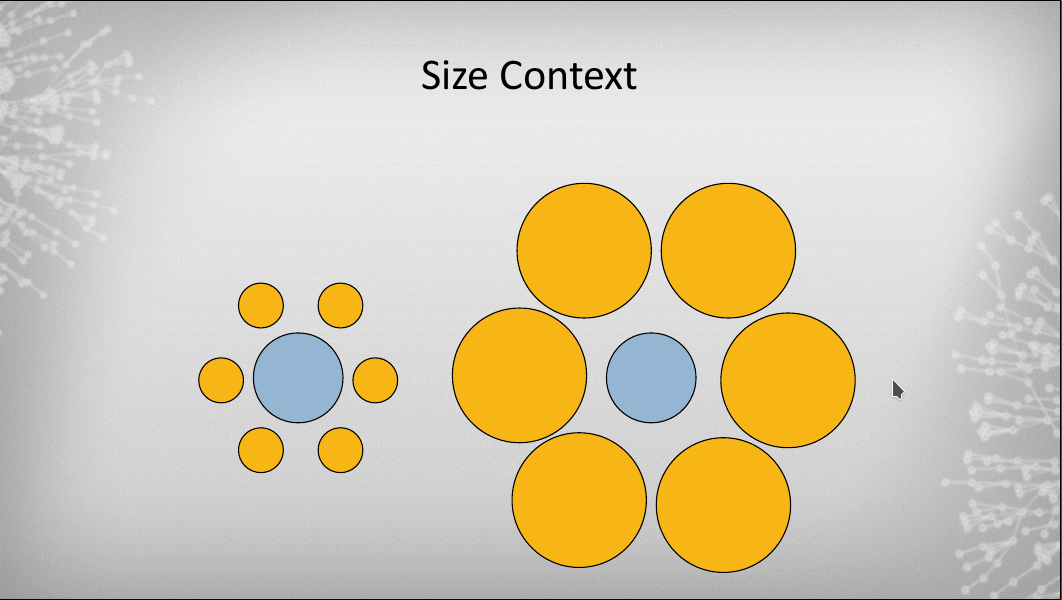
\includegraphics{images/size_context.png} In the context of color, two
identical color may seems one darker than another depends on any
surrounding colors. 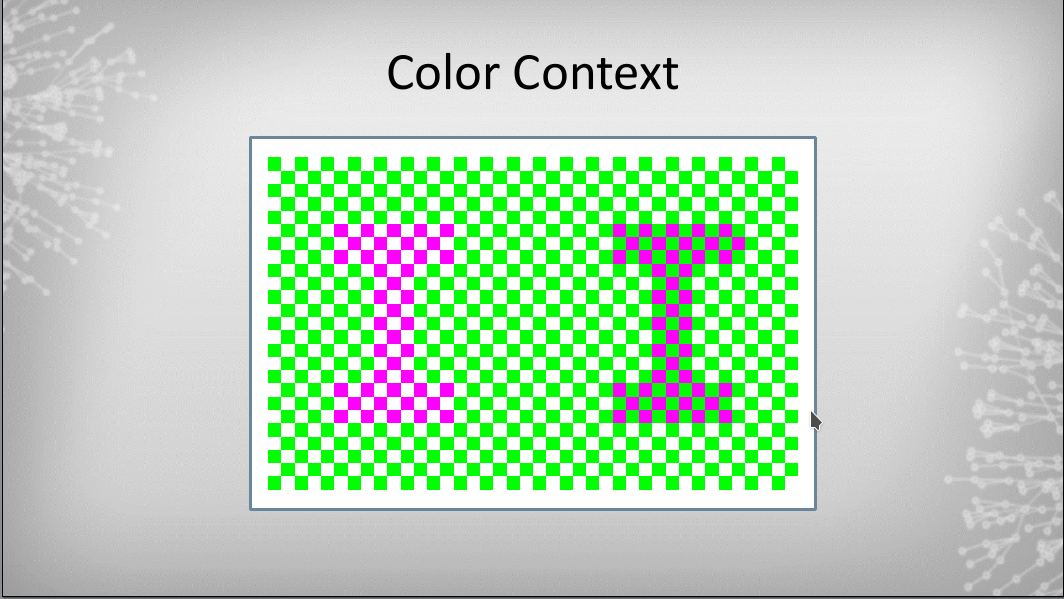
\includegraphics{images/color_context.png}

So, that is important to be consistence to choose specific context in
data visualization.

    \subsubsection{Perceiving Perspective}\label{perceiving-perspective}

Recall from section before, we can used perspective to represent 3-D
visualization on 2-D dimension object. We can used
\textbf{Foreshortening} to represent various depth of 3-D cube. We can
used \textbf{Linear Perspective} to represent object that far away
became smaller. \textbf{Size Constancy} give perception that smaller
object look farther away.

Our perception as explained before will lead us to assume that smaller
object should be farther away. So in data visualization, we need to
avoid 3-D representation as we can, and only used it if necessary.


    % Add a bibliography block to the postdoc
    
    
    
    \end{document}
